% Supplied vector figures, placed separately at their first discussion in the paper.
% Load once from main.tex; call the corresponding command in the relevant section.
% Single-column reflows preserve readable vector labels (minimum size 6.5 pt).

\newcommand{\HazBotWorkflowFigure}{%
\begin{figure}[!t]
\centering
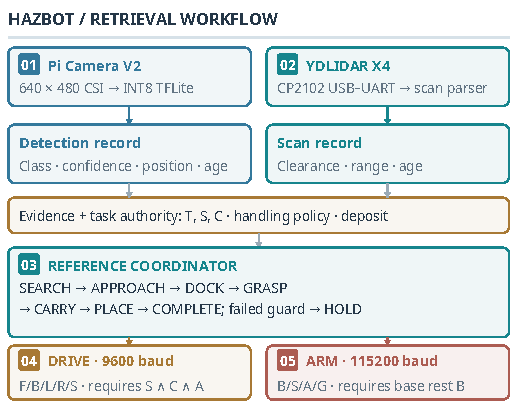
\includegraphics[width=\columnwidth]{worflow-methodology-arch/hazbot_workflow_column.pdf}
\caption{Retrieval workflow: observations and task authority feed the reference coordinator, then dedicated drive and arm controllers. Guards follow Eqs.~\ref{eq:baseguard}--\ref{eq:armguard}. Base-rest, grip and release feedback remains to be instrumented.}
\label{fig:workflow}
\end{figure}%
}

\newcommand{\HazBotMethodologyFigure}{%
\begin{figure}[!t]
\centering
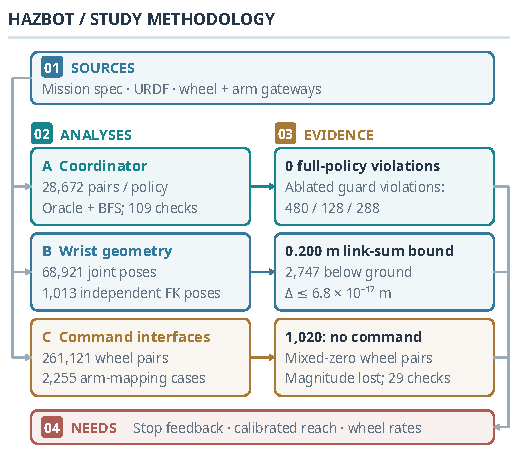
\includegraphics[width=\columnwidth]{worflow-methodology-arch/hazbot_methodology_column.pdf}
\caption{Study methodology: four source artifacts feed three offline analyses and their integration findings. The studies execute the reference model, source-isolated command logic and URDF geometry; they do not operate the robot, ROS nodes, serial hardware or detector.}
\label{fig:methodology}
\end{figure}%
}

\newcommand{\HazBotVerificationFigure}{%
\begin{figure}[!t]
\centering
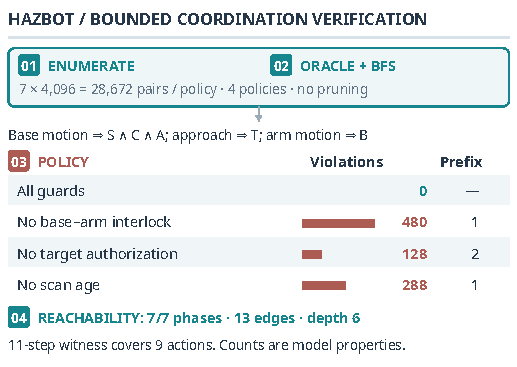
\includegraphics[width=\columnwidth]{worflow-methodology-arch/hazbot_verification_column.pdf}
\caption{Bounded verification: all phase--observation pairs are checked against an independent oracle. Prefix length counts observations to the first violating output. Reachability concerns the full policy; counts describe model properties, not robot failure rates.}
\label{fig:verification}
\end{figure}%
}
